\documentclass[twoside]{book}

% Packages required by doxygen
\usepackage{fixltx2e}
\usepackage{calc}
\usepackage{doxygen}
\usepackage[export]{adjustbox} % also loads graphicx
\usepackage{graphicx}
\usepackage[utf8]{inputenc}
\usepackage{makeidx}
\usepackage{multicol}
\usepackage{multirow}
\PassOptionsToPackage{warn}{textcomp}
\usepackage{textcomp}
\usepackage[nointegrals]{wasysym}
\usepackage[table]{xcolor}

% Font selection
\usepackage[T1]{fontenc}
\usepackage[scaled=.90]{helvet}
\usepackage{courier}
\usepackage{amssymb}
\usepackage{sectsty}
\renewcommand{\familydefault}{\sfdefault}
\allsectionsfont{%
  \fontseries{bc}\selectfont%
  \color{darkgray}%
}
\renewcommand{\DoxyLabelFont}{%
  \fontseries{bc}\selectfont%
  \color{darkgray}%
}
\newcommand{\+}{\discretionary{\mbox{\scriptsize$\hookleftarrow$}}{}{}}

% Page & text layout
\usepackage{geometry}
\geometry{%
  a4paper,%
  top=2.5cm,%
  bottom=2.5cm,%
  left=2.5cm,%
  right=2.5cm%
}
\tolerance=750
\hfuzz=15pt
\hbadness=750
\setlength{\emergencystretch}{15pt}
\setlength{\parindent}{0cm}
\setlength{\parskip}{0.2cm}
\makeatletter
\renewcommand{\paragraph}{%
  \@startsection{paragraph}{4}{0ex}{-1.0ex}{1.0ex}{%
    \normalfont\normalsize\bfseries\SS@parafont%
  }%
}
\renewcommand{\subparagraph}{%
  \@startsection{subparagraph}{5}{0ex}{-1.0ex}{1.0ex}{%
    \normalfont\normalsize\bfseries\SS@subparafont%
  }%
}
\makeatother

% Headers & footers
\usepackage{fancyhdr}
\pagestyle{fancyplain}
\fancyhead[LE]{\fancyplain{}{\bfseries\thepage}}
\fancyhead[CE]{\fancyplain{}{}}
\fancyhead[RE]{\fancyplain{}{\bfseries\leftmark}}
\fancyhead[LO]{\fancyplain{}{\bfseries\rightmark}}
\fancyhead[CO]{\fancyplain{}{}}
\fancyhead[RO]{\fancyplain{}{\bfseries\thepage}}
\fancyfoot[LE]{\fancyplain{}{}}
\fancyfoot[CE]{\fancyplain{}{}}
\fancyfoot[RE]{\fancyplain{}{\bfseries\scriptsize Generated on Sun Nov 15 2015 21\+:00\+:53 for My Project by Doxygen }}
\fancyfoot[LO]{\fancyplain{}{\bfseries\scriptsize Generated on Sun Nov 15 2015 21\+:00\+:53 for My Project by Doxygen }}
\fancyfoot[CO]{\fancyplain{}{}}
\fancyfoot[RO]{\fancyplain{}{}}
\renewcommand{\footrulewidth}{0.4pt}
\renewcommand{\chaptermark}[1]{%
  \markboth{#1}{}%
}
\renewcommand{\sectionmark}[1]{%
  \markright{\thesection\ #1}%
}

% Indices & bibliography
\usepackage{natbib}
\usepackage[titles]{tocloft}
\setcounter{tocdepth}{3}
\setcounter{secnumdepth}{5}
\makeindex

% Hyperlinks (required, but should be loaded last)
\usepackage{ifpdf}
\ifpdf
  \usepackage[pdftex,pagebackref=true]{hyperref}
\else
  \usepackage[ps2pdf,pagebackref=true]{hyperref}
\fi
\hypersetup{%
  colorlinks=true,%
  linkcolor=blue,%
  citecolor=blue,%
  unicode%
}

% Custom commands
\newcommand{\clearemptydoublepage}{%
  \newpage{\pagestyle{empty}\cleardoublepage}%
}


%===== C O N T E N T S =====

\begin{document}

% Titlepage & ToC
\hypersetup{pageanchor=false,
             bookmarks=true,
             bookmarksnumbered=true,
             pdfencoding=unicode
            }
\pagenumbering{roman}
\begin{titlepage}
\vspace*{7cm}
\begin{center}%
{\Large My Project }\\
\vspace*{1cm}
{\large Generated by Doxygen 1.8.10}\\
\vspace*{0.5cm}
{\small Sun Nov 15 2015 21:00:53}\\
\end{center}
\end{titlepage}
\clearemptydoublepage
\tableofcontents
\clearemptydoublepage
\pagenumbering{arabic}
\hypersetup{pageanchor=true}

%--- Begin generated contents ---
\chapter{Hierarchical Index}
\section{Class Hierarchy}
This inheritance list is sorted roughly, but not completely, alphabetically\+:\begin{DoxyCompactList}
\item \contentsline{section}{Machine}{\pageref{class_machine}}{}
\begin{DoxyCompactList}
\item \contentsline{section}{Bike}{\pageref{class_bike}}{}
\item \contentsline{section}{Squat\+\_\+\+Rack}{\pageref{class_squat___rack}}{}
\item \contentsline{section}{Treadmill}{\pageref{class_treadmill}}{}
\end{DoxyCompactList}
\item \contentsline{section}{Machine\+Factory}{\pageref{class_machine_factory}}{}
\end{DoxyCompactList}

\chapter{Class Index}
\section{Class List}
Here are the classes, structs, unions and interfaces with brief descriptions\+:\begin{DoxyCompactList}
\item\contentsline{section}{\hyperlink{class_bike}{Bike} \\*\hyperlink{class_bike}{Bike} }{\pageref{class_bike}}{}
\item\contentsline{section}{\hyperlink{class_machine}{Machine} \\*\hyperlink{class_machine}{Machine} }{\pageref{class_machine}}{}
\item\contentsline{section}{\hyperlink{class_machine_factory}{Machine\+Factory} \\*\hyperlink{class_machine}{Machine} Factory class }{\pageref{class_machine_factory}}{}
\item\contentsline{section}{\hyperlink{class_squat___rack}{Squat\+\_\+\+Rack} \\*Squat Rack }{\pageref{class_squat___rack}}{}
\item\contentsline{section}{\hyperlink{class_treadmill}{Treadmill} \\*\hyperlink{class_treadmill}{Treadmill} }{\pageref{class_treadmill}}{}
\end{DoxyCompactList}

\chapter{Class Documentation}
\hypertarget{class_bike}{}\section{Bike Class Reference}
\label{class_bike}\index{Bike@{Bike}}


\hyperlink{class_bike}{Bike}.  




{\ttfamily \#include $<$Bike.\+h$>$}

Inheritance diagram for Bike\+:\begin{figure}[H]
\begin{center}
\leavevmode
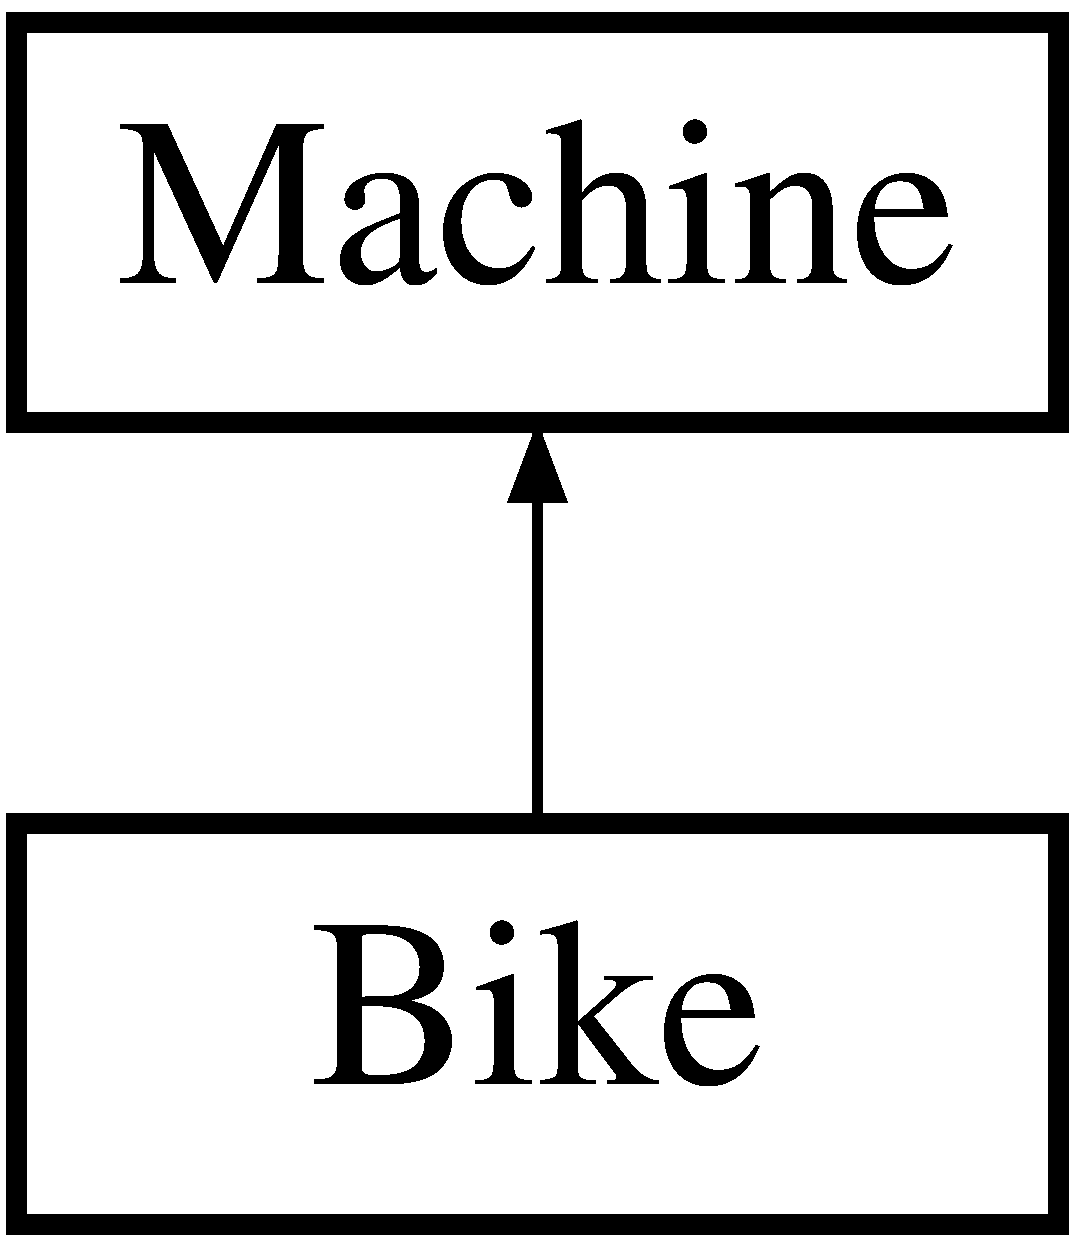
\includegraphics[height=2.000000cm]{class_bike}
\end{center}
\end{figure}
\subsection*{Public Member Functions}
\begin{DoxyCompactItemize}
\item 
\hyperlink{class_bike_ad939a72af830128eef933a6aae2b6a67}{Bike} (string \+\_\+name)
\begin{DoxyCompactList}\small\item\em Constructor for \hyperlink{class_bike}{Bike} prototype. \end{DoxyCompactList}\item 
\hyperlink{class_bike_a7707ee6f2cc666cd7eb6f076779de089}{Bike} (const \hyperlink{class_bike}{Bike} \&copy)
\begin{DoxyCompactList}\small\item\em Constructor for \hyperlink{class_bike}{Bike} copies. \end{DoxyCompactList}\item 
\hypertarget{class_bike_aaa9b2dad18f1576519a0d9c7afe425b7}{}\hyperlink{class_bike_aaa9b2dad18f1576519a0d9c7afe425b7}{$\sim$\+Bike} ()\label{class_bike_aaa9b2dad18f1576519a0d9c7afe425b7}

\begin{DoxyCompactList}\small\item\em Destructor for \hyperlink{class_bike}{Bike}. \end{DoxyCompactList}\item 
\hyperlink{class_machine}{Machine} $\ast$ \hyperlink{class_bike_afa7db5dc0a537829e8f5ec0d0b241b3f}{clone} ()
\begin{DoxyCompactList}\small\item\em \hyperlink{class_bike}{Bike} clone function. \end{DoxyCompactList}\item 
void \hyperlink{class_bike_aabdef60bdefd4d4d07a3abdcfc83e6f4}{print} ()
\begin{DoxyCompactList}\small\item\em Print name function. \end{DoxyCompactList}\item 
void \hyperlink{class_bike_a2b74c0aad112737a663bcc85bd5f7712}{change\+Name} (string)
\begin{DoxyCompactList}\small\item\em Change name function. \end{DoxyCompactList}\end{DoxyCompactItemize}


\subsection{Detailed Description}
\hyperlink{class_bike}{Bike}. 

This is a derived class of \hyperlink{class_machine}{Machine}. It is used to create a new \hyperlink{class_bike}{Bike}. 

\subsection{Constructor \& Destructor Documentation}
\hypertarget{class_bike_ad939a72af830128eef933a6aae2b6a67}{}\index{Bike@{Bike}!Bike@{Bike}}
\index{Bike@{Bike}!Bike@{Bike}}
\subsubsection[{Bike(string \+\_\+name)}]{\setlength{\rightskip}{0pt plus 5cm}Bike\+::\+Bike (
\begin{DoxyParamCaption}
\item[{string}]{\+\_\+name}
\end{DoxyParamCaption}
)}\label{class_bike_ad939a72af830128eef933a6aae2b6a67}


Constructor for \hyperlink{class_bike}{Bike} prototype. 

every new \hyperlink{class_bike}{Bike} created will be a copy of this. \hypertarget{class_bike_a7707ee6f2cc666cd7eb6f076779de089}{}\index{Bike@{Bike}!Bike@{Bike}}
\index{Bike@{Bike}!Bike@{Bike}}
\subsubsection[{Bike(const Bike \&copy)}]{\setlength{\rightskip}{0pt plus 5cm}Bike\+::\+Bike (
\begin{DoxyParamCaption}
\item[{const {\bf Bike} \&}]{copy}
\end{DoxyParamCaption}
)}\label{class_bike_a7707ee6f2cc666cd7eb6f076779de089}


Constructor for \hyperlink{class_bike}{Bike} copies. 

every new \hyperlink{class_bike}{Bike} created will use this constructor. It will copy the attributes of the prototype \hyperlink{class_bike}{Bike}. 

\subsection{Member Function Documentation}
\hypertarget{class_bike_a2b74c0aad112737a663bcc85bd5f7712}{}\index{Bike@{Bike}!change\+Name@{change\+Name}}
\index{change\+Name@{change\+Name}!Bike@{Bike}}
\subsubsection[{change\+Name(string)}]{\setlength{\rightskip}{0pt plus 5cm}void Bike\+::change\+Name (
\begin{DoxyParamCaption}
\item[{string}]{new\+Name}
\end{DoxyParamCaption}
)\hspace{0.3cm}{\ttfamily [virtual]}}\label{class_bike_a2b74c0aad112737a663bcc85bd5f7712}


Change name function. 

Changes the \hyperlink{class_bike}{Bike}\textquotesingle{}s name. 

Implements \hyperlink{class_machine}{Machine}.

\hypertarget{class_bike_afa7db5dc0a537829e8f5ec0d0b241b3f}{}\index{Bike@{Bike}!clone@{clone}}
\index{clone@{clone}!Bike@{Bike}}
\subsubsection[{clone()}]{\setlength{\rightskip}{0pt plus 5cm}{\bf Machine} $\ast$ Bike\+::clone (
\begin{DoxyParamCaption}
{}
\end{DoxyParamCaption}
)\hspace{0.3cm}{\ttfamily [virtual]}}\label{class_bike_afa7db5dc0a537829e8f5ec0d0b241b3f}


\hyperlink{class_bike}{Bike} clone function. 

It will return a new copy of the prototype \hyperlink{class_bike}{Bike} using the \hyperlink{class_bike}{Bike} copy constructor. 

Implements \hyperlink{class_machine}{Machine}.

\hypertarget{class_bike_aabdef60bdefd4d4d07a3abdcfc83e6f4}{}\index{Bike@{Bike}!print@{print}}
\index{print@{print}!Bike@{Bike}}
\subsubsection[{print()}]{\setlength{\rightskip}{0pt plus 5cm}void Bike\+::print (
\begin{DoxyParamCaption}
{}
\end{DoxyParamCaption}
)\hspace{0.3cm}{\ttfamily [virtual]}}\label{class_bike_aabdef60bdefd4d4d07a3abdcfc83e6f4}


Print name function. 

It will print the name of the \hyperlink{class_bike}{Bike}. 

Implements \hyperlink{class_machine}{Machine}.



The documentation for this class was generated from the following files\+:\begin{DoxyCompactItemize}
\item 
Seng330\+A2/\+Seng330\+A2/Bike.\+h\item 
Seng330\+A2/\+Seng330\+A2/Bike.\+cpp\end{DoxyCompactItemize}

\hypertarget{class_machine}{}\section{Machine Class Reference}
\label{class_machine}\index{Machine@{Machine}}


\hyperlink{class_machine}{Machine}.  




{\ttfamily \#include $<$Machine.\+h$>$}

Inheritance diagram for Machine\+:\begin{figure}[H]
\begin{center}
\leavevmode
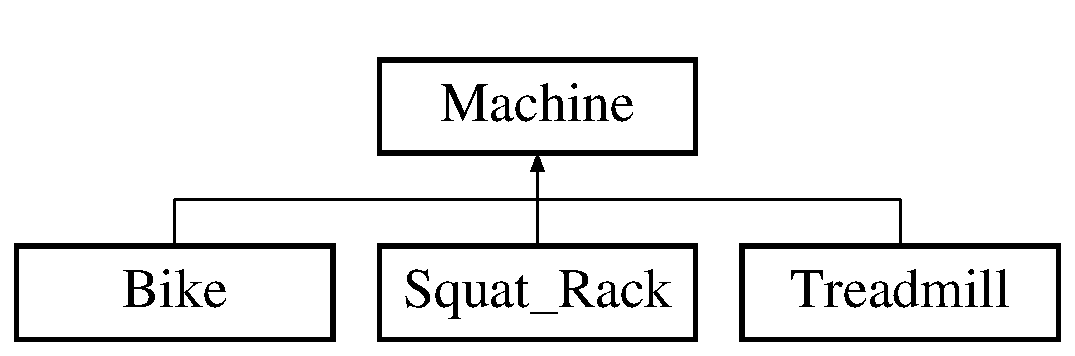
\includegraphics[height=2.000000cm]{class_machine}
\end{center}
\end{figure}
\subsection*{Public Member Functions}
\begin{DoxyCompactItemize}
\item 
\hypertarget{class_machine_a2175bf6ebeb5b3d83c35534de8e5dc3d}{}virtual \hyperlink{class_machine}{Machine} $\ast$ {\bfseries clone} ()=0\label{class_machine_a2175bf6ebeb5b3d83c35534de8e5dc3d}

\item 
\hypertarget{class_machine_a0fab59a376dd6cd5708a0d95fab48d0c}{}virtual void {\bfseries print} ()=0\label{class_machine_a0fab59a376dd6cd5708a0d95fab48d0c}

\item 
\hypertarget{class_machine_a3cc1f418d54f49ac547b08f5cbb01846}{}virtual void {\bfseries change\+Name} (string)=0\label{class_machine_a3cc1f418d54f49ac547b08f5cbb01846}

\end{DoxyCompactItemize}


\subsection{Detailed Description}
\hyperlink{class_machine}{Machine}. 

This is the base Prototype for all the different types of machines. 

The documentation for this class was generated from the following files\+:\begin{DoxyCompactItemize}
\item 
Seng330\+A2/\+Seng330\+A2/Machine.\+h\item 
Seng330\+A2/\+Seng330\+A2/Machine.\+cpp\end{DoxyCompactItemize}

\hypertarget{class_machine_factory}{}\section{Machine\+Factory Class Reference}
\label{class_machine_factory}\index{Machine\+Factory@{Machine\+Factory}}


\hyperlink{class_machine}{Machine} Factory class.  




{\ttfamily \#include $<$Machine\+Factory.\+h$>$}

\subsection*{Public Member Functions}
\begin{DoxyCompactItemize}
\item 
\hyperlink{class_machine_factory_ae585766b671db16d78d4d580d80261f1}{Machine\+Factory} ()
\begin{DoxyCompactList}\small\item\em \hyperlink{class_machine_factory}{Machine\+Factory} constructor. \end{DoxyCompactList}\item 
\hyperlink{class_machine_factory_a098ac5638472df854885d9973444daf5}{$\sim$\+Machine\+Factory} ()
\begin{DoxyCompactList}\small\item\em \hyperlink{class_machine_factory}{Machine\+Factory} Destructor. \end{DoxyCompactList}\item 
\hyperlink{class_machine}{Machine} $\ast$ \hyperlink{class_machine_factory_a1ce75d92c7342129acab9384560aa3b5}{create\+Machine} (M\+A\+C\+H\+I\+N\+E\+\_\+\+T\+Y\+P\+E type)
\begin{DoxyCompactList}\small\item\em \hyperlink{class_machine}{Machine} creation function. \end{DoxyCompactList}\end{DoxyCompactItemize}


\subsection{Detailed Description}
\hyperlink{class_machine}{Machine} Factory class. 

This creates the prototype objects and has a method for cloning new objects from the prototype. 

\subsection{Constructor \& Destructor Documentation}
\hypertarget{class_machine_factory_ae585766b671db16d78d4d580d80261f1}{}\index{Machine\+Factory@{Machine\+Factory}!Machine\+Factory@{Machine\+Factory}}
\index{Machine\+Factory@{Machine\+Factory}!Machine\+Factory@{Machine\+Factory}}
\subsubsection[{Machine\+Factory()}]{\setlength{\rightskip}{0pt plus 5cm}Machine\+Factory\+::\+Machine\+Factory (
\begin{DoxyParamCaption}
{}
\end{DoxyParamCaption}
)}\label{class_machine_factory_ae585766b671db16d78d4d580d80261f1}


\hyperlink{class_machine_factory}{Machine\+Factory} constructor. 

This will create a new \hyperlink{class_machine}{Machine} Factory and the prototype objects for each different machine. \hypertarget{class_machine_factory_a098ac5638472df854885d9973444daf5}{}\index{Machine\+Factory@{Machine\+Factory}!````~Machine\+Factory@{$\sim$\+Machine\+Factory}}
\index{````~Machine\+Factory@{$\sim$\+Machine\+Factory}!Machine\+Factory@{Machine\+Factory}}
\subsubsection[{$\sim$\+Machine\+Factory()}]{\setlength{\rightskip}{0pt plus 5cm}Machine\+Factory\+::$\sim$\+Machine\+Factory (
\begin{DoxyParamCaption}
{}
\end{DoxyParamCaption}
)}\label{class_machine_factory_a098ac5638472df854885d9973444daf5}


\hyperlink{class_machine_factory}{Machine\+Factory} Destructor. 

This will remove the \hyperlink{class_machine}{Machine} Factory and the prototype objects for each different machine when they are no longer needed. 

\subsection{Member Function Documentation}
\hypertarget{class_machine_factory_a1ce75d92c7342129acab9384560aa3b5}{}\index{Machine\+Factory@{Machine\+Factory}!create\+Machine@{create\+Machine}}
\index{create\+Machine@{create\+Machine}!Machine\+Factory@{Machine\+Factory}}
\subsubsection[{create\+Machine(\+M\+A\+C\+H\+I\+N\+E\+\_\+\+T\+Y\+P\+E type)}]{\setlength{\rightskip}{0pt plus 5cm}{\bf Machine} $\ast$ Machine\+Factory\+::create\+Machine (
\begin{DoxyParamCaption}
\item[{M\+A\+C\+H\+I\+N\+E\+\_\+\+T\+Y\+P\+E}]{type}
\end{DoxyParamCaption}
)}\label{class_machine_factory_a1ce75d92c7342129acab9384560aa3b5}


\hyperlink{class_machine}{Machine} creation function. 

This will create a new machine by copying the prototype and returning it as a new machine. 

The documentation for this class was generated from the following files\+:\begin{DoxyCompactItemize}
\item 
Seng330\+A2/\+Seng330\+A2/Machine\+Factory.\+h\item 
Seng330\+A2/\+Seng330\+A2/Machine\+Factory.\+cpp\end{DoxyCompactItemize}

\hypertarget{class_squat___rack}{}\section{Squat\+\_\+\+Rack Class Reference}
\label{class_squat___rack}\index{Squat\+\_\+\+Rack@{Squat\+\_\+\+Rack}}


Squat Rack.  




{\ttfamily \#include $<$Squat\+Rack.\+h$>$}

Inheritance diagram for Squat\+\_\+\+Rack\+:\begin{figure}[H]
\begin{center}
\leavevmode
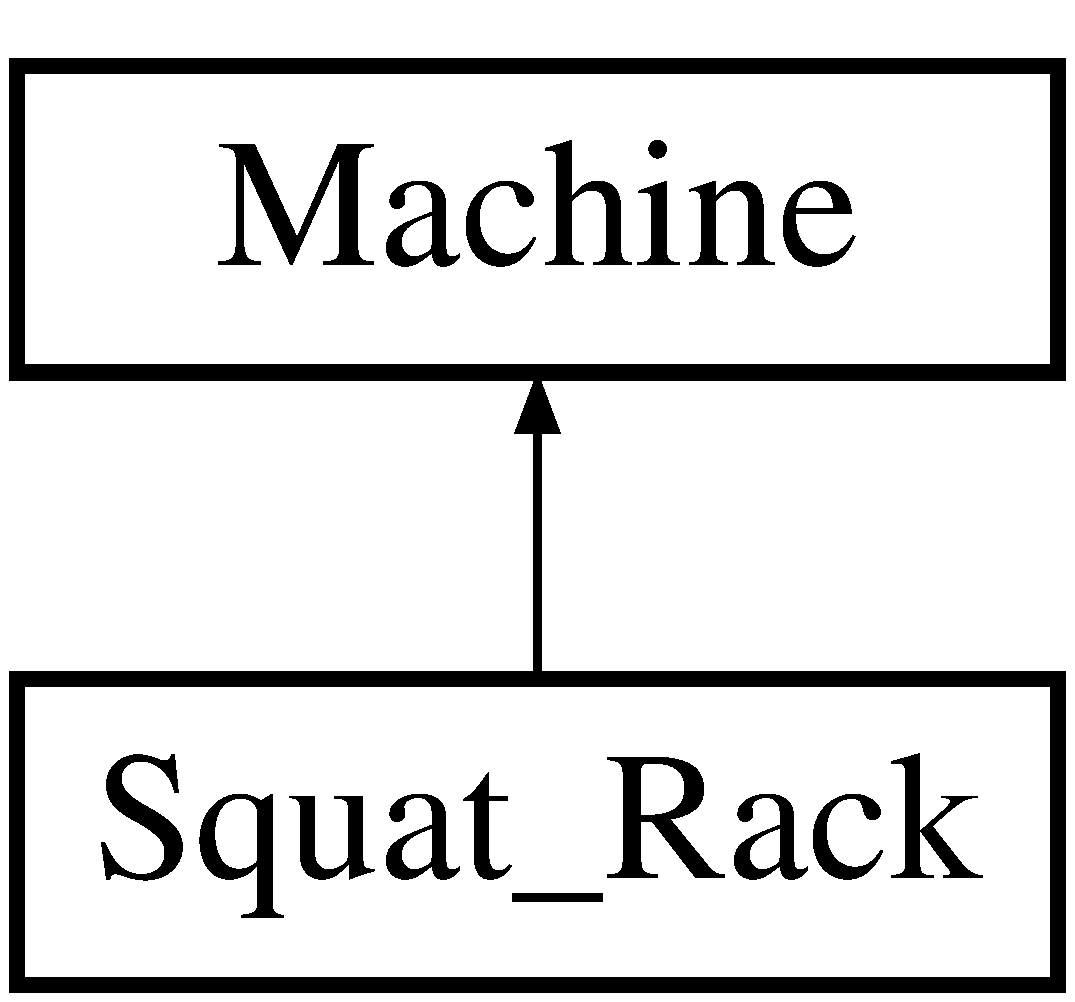
\includegraphics[height=2.000000cm]{class_squat___rack}
\end{center}
\end{figure}
\subsection*{Public Member Functions}
\begin{DoxyCompactItemize}
\item 
\hyperlink{class_squat___rack_a7914ba2400f02ef59e49a246c518428b}{Squat\+\_\+\+Rack} (string \+\_\+name)
\begin{DoxyCompactList}\small\item\em Constructor for Squat Rack prototype. \end{DoxyCompactList}\item 
\hyperlink{class_squat___rack_a17d776321a5c097a894fb703829a433e}{Squat\+\_\+\+Rack} (const \hyperlink{class_squat___rack}{Squat\+\_\+\+Rack} \&copy)
\begin{DoxyCompactList}\small\item\em Constructor for Squat Rack copies. \end{DoxyCompactList}\item 
\hypertarget{class_squat___rack_af5d168b52a31ca3129f8864991137440}{}\hyperlink{class_squat___rack_af5d168b52a31ca3129f8864991137440}{$\sim$\+Squat\+\_\+\+Rack} ()\label{class_squat___rack_af5d168b52a31ca3129f8864991137440}

\begin{DoxyCompactList}\small\item\em Destructor for Squat Rack. \end{DoxyCompactList}\item 
\hyperlink{class_machine}{Machine} $\ast$ \hyperlink{class_squat___rack_a6eceabbfc212c9d513a6eb335da43916}{clone} ()
\begin{DoxyCompactList}\small\item\em Squat Rack clone function. \end{DoxyCompactList}\item 
void \hyperlink{class_squat___rack_a63321b3a00a68f82c42d5713ac01f24f}{print} ()
\begin{DoxyCompactList}\small\item\em Print name function. \end{DoxyCompactList}\item 
void \hyperlink{class_squat___rack_ad309d281458a753255ed8c4c6f5a24d4}{change\+Name} (string)
\begin{DoxyCompactList}\small\item\em Change name function. \end{DoxyCompactList}\end{DoxyCompactItemize}


\subsection{Detailed Description}
Squat Rack. 

This is a derived class of \hyperlink{class_machine}{Machine}. It is used to create a new Squat Rack. 

\subsection{Constructor \& Destructor Documentation}
\hypertarget{class_squat___rack_a7914ba2400f02ef59e49a246c518428b}{}\index{Squat\+\_\+\+Rack@{Squat\+\_\+\+Rack}!Squat\+\_\+\+Rack@{Squat\+\_\+\+Rack}}
\index{Squat\+\_\+\+Rack@{Squat\+\_\+\+Rack}!Squat\+\_\+\+Rack@{Squat\+\_\+\+Rack}}
\subsubsection[{Squat\+\_\+\+Rack(string \+\_\+name)}]{\setlength{\rightskip}{0pt plus 5cm}Squat\+\_\+\+Rack\+::\+Squat\+\_\+\+Rack (
\begin{DoxyParamCaption}
\item[{string}]{\+\_\+name}
\end{DoxyParamCaption}
)}\label{class_squat___rack_a7914ba2400f02ef59e49a246c518428b}


Constructor for Squat Rack prototype. 

every new Squat Rack created will be a copy of this. \hypertarget{class_squat___rack_a17d776321a5c097a894fb703829a433e}{}\index{Squat\+\_\+\+Rack@{Squat\+\_\+\+Rack}!Squat\+\_\+\+Rack@{Squat\+\_\+\+Rack}}
\index{Squat\+\_\+\+Rack@{Squat\+\_\+\+Rack}!Squat\+\_\+\+Rack@{Squat\+\_\+\+Rack}}
\subsubsection[{Squat\+\_\+\+Rack(const Squat\+\_\+\+Rack \&copy)}]{\setlength{\rightskip}{0pt plus 5cm}Squat\+\_\+\+Rack\+::\+Squat\+\_\+\+Rack (
\begin{DoxyParamCaption}
\item[{const {\bf Squat\+\_\+\+Rack} \&}]{copy}
\end{DoxyParamCaption}
)}\label{class_squat___rack_a17d776321a5c097a894fb703829a433e}


Constructor for Squat Rack copies. 

every new Squat Rack created will use this constructor. It will copy the attributes of the prototype Squat Rack. 

\subsection{Member Function Documentation}
\hypertarget{class_squat___rack_ad309d281458a753255ed8c4c6f5a24d4}{}\index{Squat\+\_\+\+Rack@{Squat\+\_\+\+Rack}!change\+Name@{change\+Name}}
\index{change\+Name@{change\+Name}!Squat\+\_\+\+Rack@{Squat\+\_\+\+Rack}}
\subsubsection[{change\+Name(string)}]{\setlength{\rightskip}{0pt plus 5cm}void Squat\+\_\+\+Rack\+::change\+Name (
\begin{DoxyParamCaption}
\item[{string}]{new\+Name}
\end{DoxyParamCaption}
)\hspace{0.3cm}{\ttfamily [virtual]}}\label{class_squat___rack_ad309d281458a753255ed8c4c6f5a24d4}


Change name function. 

Changes the Squat rack\textquotesingle{}s name. 

Implements \hyperlink{class_machine}{Machine}.

\hypertarget{class_squat___rack_a6eceabbfc212c9d513a6eb335da43916}{}\index{Squat\+\_\+\+Rack@{Squat\+\_\+\+Rack}!clone@{clone}}
\index{clone@{clone}!Squat\+\_\+\+Rack@{Squat\+\_\+\+Rack}}
\subsubsection[{clone()}]{\setlength{\rightskip}{0pt plus 5cm}{\bf Machine} $\ast$ Squat\+\_\+\+Rack\+::clone (
\begin{DoxyParamCaption}
{}
\end{DoxyParamCaption}
)\hspace{0.3cm}{\ttfamily [virtual]}}\label{class_squat___rack_a6eceabbfc212c9d513a6eb335da43916}


Squat Rack clone function. 

It will return a new copy of the prototype Squat Rack using the Squat Rack copy constructor. 

Implements \hyperlink{class_machine}{Machine}.

\hypertarget{class_squat___rack_a63321b3a00a68f82c42d5713ac01f24f}{}\index{Squat\+\_\+\+Rack@{Squat\+\_\+\+Rack}!print@{print}}
\index{print@{print}!Squat\+\_\+\+Rack@{Squat\+\_\+\+Rack}}
\subsubsection[{print()}]{\setlength{\rightskip}{0pt plus 5cm}void Squat\+\_\+\+Rack\+::print (
\begin{DoxyParamCaption}
{}
\end{DoxyParamCaption}
)\hspace{0.3cm}{\ttfamily [virtual]}}\label{class_squat___rack_a63321b3a00a68f82c42d5713ac01f24f}


Print name function. 

It will print the name of the Squat Rack. 

Implements \hyperlink{class_machine}{Machine}.



The documentation for this class was generated from the following files\+:\begin{DoxyCompactItemize}
\item 
Seng330\+A2/\+Seng330\+A2/Squat\+Rack.\+h\item 
Seng330\+A2/\+Seng330\+A2/Squat\+Rack.\+cpp\end{DoxyCompactItemize}

\hypertarget{class_treadmill}{}\section{Treadmill Class Reference}
\label{class_treadmill}\index{Treadmill@{Treadmill}}


\hyperlink{class_treadmill}{Treadmill}.  




{\ttfamily \#include $<$Treadmill.\+h$>$}

Inheritance diagram for Treadmill\+:\begin{figure}[H]
\begin{center}
\leavevmode
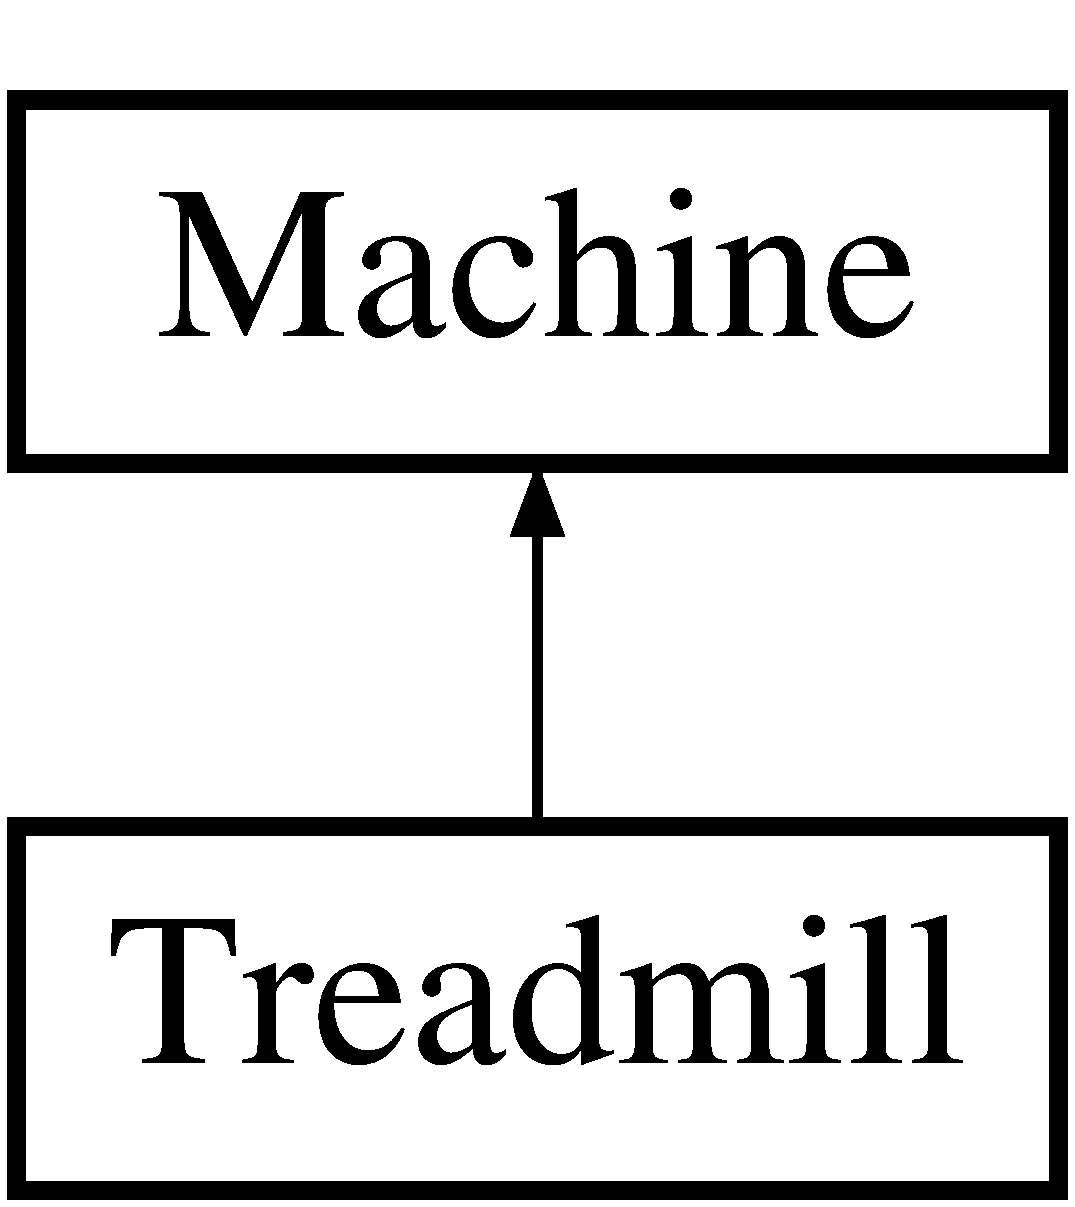
\includegraphics[height=2.000000cm]{class_treadmill}
\end{center}
\end{figure}
\subsection*{Public Member Functions}
\begin{DoxyCompactItemize}
\item 
\hyperlink{class_treadmill_a4f25c125cffee47960cedd2f003c61bd}{Treadmill} (string \+\_\+name)
\begin{DoxyCompactList}\small\item\em Constructor for treadmill prototype. \end{DoxyCompactList}\item 
\hyperlink{class_treadmill_a61ab63a87accfd647c2815ca64d0a3a3}{Treadmill} (const \hyperlink{class_treadmill}{Treadmill} \&copy)
\begin{DoxyCompactList}\small\item\em Constructor for treadmill copies. \end{DoxyCompactList}\item 
\hypertarget{class_treadmill_a9269ef0174af69f96d65de8f416dca6e}{}\hyperlink{class_treadmill_a9269ef0174af69f96d65de8f416dca6e}{$\sim$\+Treadmill} ()\label{class_treadmill_a9269ef0174af69f96d65de8f416dca6e}

\begin{DoxyCompactList}\small\item\em Destructor for treadmill prototype. \end{DoxyCompactList}\item 
\hyperlink{class_machine}{Machine} $\ast$ \hyperlink{class_treadmill_a30d83dada44a2d148e8d14dcf9d8d6d6}{clone} ()
\begin{DoxyCompactList}\small\item\em \hyperlink{class_treadmill}{Treadmill} clone function. \end{DoxyCompactList}\item 
void \hyperlink{class_treadmill_a0663e09b1573550cd6241d086482e973}{print} ()
\begin{DoxyCompactList}\small\item\em Print name function. \end{DoxyCompactList}\item 
void \hyperlink{class_treadmill_a7600b2dee59e7a4f8cd37c270c4ca67f}{change\+Name} (string)
\begin{DoxyCompactList}\small\item\em Change name function. \end{DoxyCompactList}\end{DoxyCompactItemize}


\subsection{Detailed Description}
\hyperlink{class_treadmill}{Treadmill}. 

This is a derived class of \hyperlink{class_machine}{Machine}. It is used to create a new treadmill. 

\subsection{Constructor \& Destructor Documentation}
\hypertarget{class_treadmill_a4f25c125cffee47960cedd2f003c61bd}{}\index{Treadmill@{Treadmill}!Treadmill@{Treadmill}}
\index{Treadmill@{Treadmill}!Treadmill@{Treadmill}}
\subsubsection[{Treadmill(string \+\_\+name)}]{\setlength{\rightskip}{0pt plus 5cm}Treadmill\+::\+Treadmill (
\begin{DoxyParamCaption}
\item[{string}]{\+\_\+name}
\end{DoxyParamCaption}
)}\label{class_treadmill_a4f25c125cffee47960cedd2f003c61bd}


Constructor for treadmill prototype. 

every new treadmill created will be a copy of this. \hypertarget{class_treadmill_a61ab63a87accfd647c2815ca64d0a3a3}{}\index{Treadmill@{Treadmill}!Treadmill@{Treadmill}}
\index{Treadmill@{Treadmill}!Treadmill@{Treadmill}}
\subsubsection[{Treadmill(const Treadmill \&copy)}]{\setlength{\rightskip}{0pt plus 5cm}Treadmill\+::\+Treadmill (
\begin{DoxyParamCaption}
\item[{const {\bf Treadmill} \&}]{copy}
\end{DoxyParamCaption}
)}\label{class_treadmill_a61ab63a87accfd647c2815ca64d0a3a3}


Constructor for treadmill copies. 

every new treadmill created will use this constructor. It will copy the attributes of the prototype treadmill. 

\subsection{Member Function Documentation}
\hypertarget{class_treadmill_a7600b2dee59e7a4f8cd37c270c4ca67f}{}\index{Treadmill@{Treadmill}!change\+Name@{change\+Name}}
\index{change\+Name@{change\+Name}!Treadmill@{Treadmill}}
\subsubsection[{change\+Name(string)}]{\setlength{\rightskip}{0pt plus 5cm}void Treadmill\+::change\+Name (
\begin{DoxyParamCaption}
\item[{string}]{new\+Name}
\end{DoxyParamCaption}
)\hspace{0.3cm}{\ttfamily [virtual]}}\label{class_treadmill_a7600b2dee59e7a4f8cd37c270c4ca67f}


Change name function. 

Changes the treadmill\textquotesingle{}s name. 

Implements \hyperlink{class_machine}{Machine}.

\hypertarget{class_treadmill_a30d83dada44a2d148e8d14dcf9d8d6d6}{}\index{Treadmill@{Treadmill}!clone@{clone}}
\index{clone@{clone}!Treadmill@{Treadmill}}
\subsubsection[{clone()}]{\setlength{\rightskip}{0pt plus 5cm}{\bf Machine} $\ast$ Treadmill\+::clone (
\begin{DoxyParamCaption}
{}
\end{DoxyParamCaption}
)\hspace{0.3cm}{\ttfamily [virtual]}}\label{class_treadmill_a30d83dada44a2d148e8d14dcf9d8d6d6}


\hyperlink{class_treadmill}{Treadmill} clone function. 

It will return a new copy of the prototype treadmill using the treadmill copy constructor. 

Implements \hyperlink{class_machine}{Machine}.

\hypertarget{class_treadmill_a0663e09b1573550cd6241d086482e973}{}\index{Treadmill@{Treadmill}!print@{print}}
\index{print@{print}!Treadmill@{Treadmill}}
\subsubsection[{print()}]{\setlength{\rightskip}{0pt plus 5cm}void Treadmill\+::print (
\begin{DoxyParamCaption}
{}
\end{DoxyParamCaption}
)\hspace{0.3cm}{\ttfamily [virtual]}}\label{class_treadmill_a0663e09b1573550cd6241d086482e973}


Print name function. 

It will print the name of the \hyperlink{class_treadmill}{Treadmill}. 

Implements \hyperlink{class_machine}{Machine}.



The documentation for this class was generated from the following files\+:\begin{DoxyCompactItemize}
\item 
Seng330\+A2/\+Seng330\+A2/Treadmill.\+h\item 
Seng330\+A2/\+Seng330\+A2/Treadmill.\+cpp\end{DoxyCompactItemize}

%--- End generated contents ---

% Index
\backmatter
\newpage
\phantomsection
\clearemptydoublepage
\addcontentsline{toc}{chapter}{Index}
\printindex

\end{document}
